\appendix
\section{\\Title of Appendix A}
% the \\ insures the section title is centered below the phrase: AppendixA

\begin{figure}
The Risk Analysis table defines a potential set of risks that our group determined were possible to face, as setbacks to timely progression towards our finished project. For each risk, there are two potential consequences, a probability value 0 to 1, a severity value 0 to 10, an impact value (impact=probability*severity), and potential mitigation strategies.
\newline
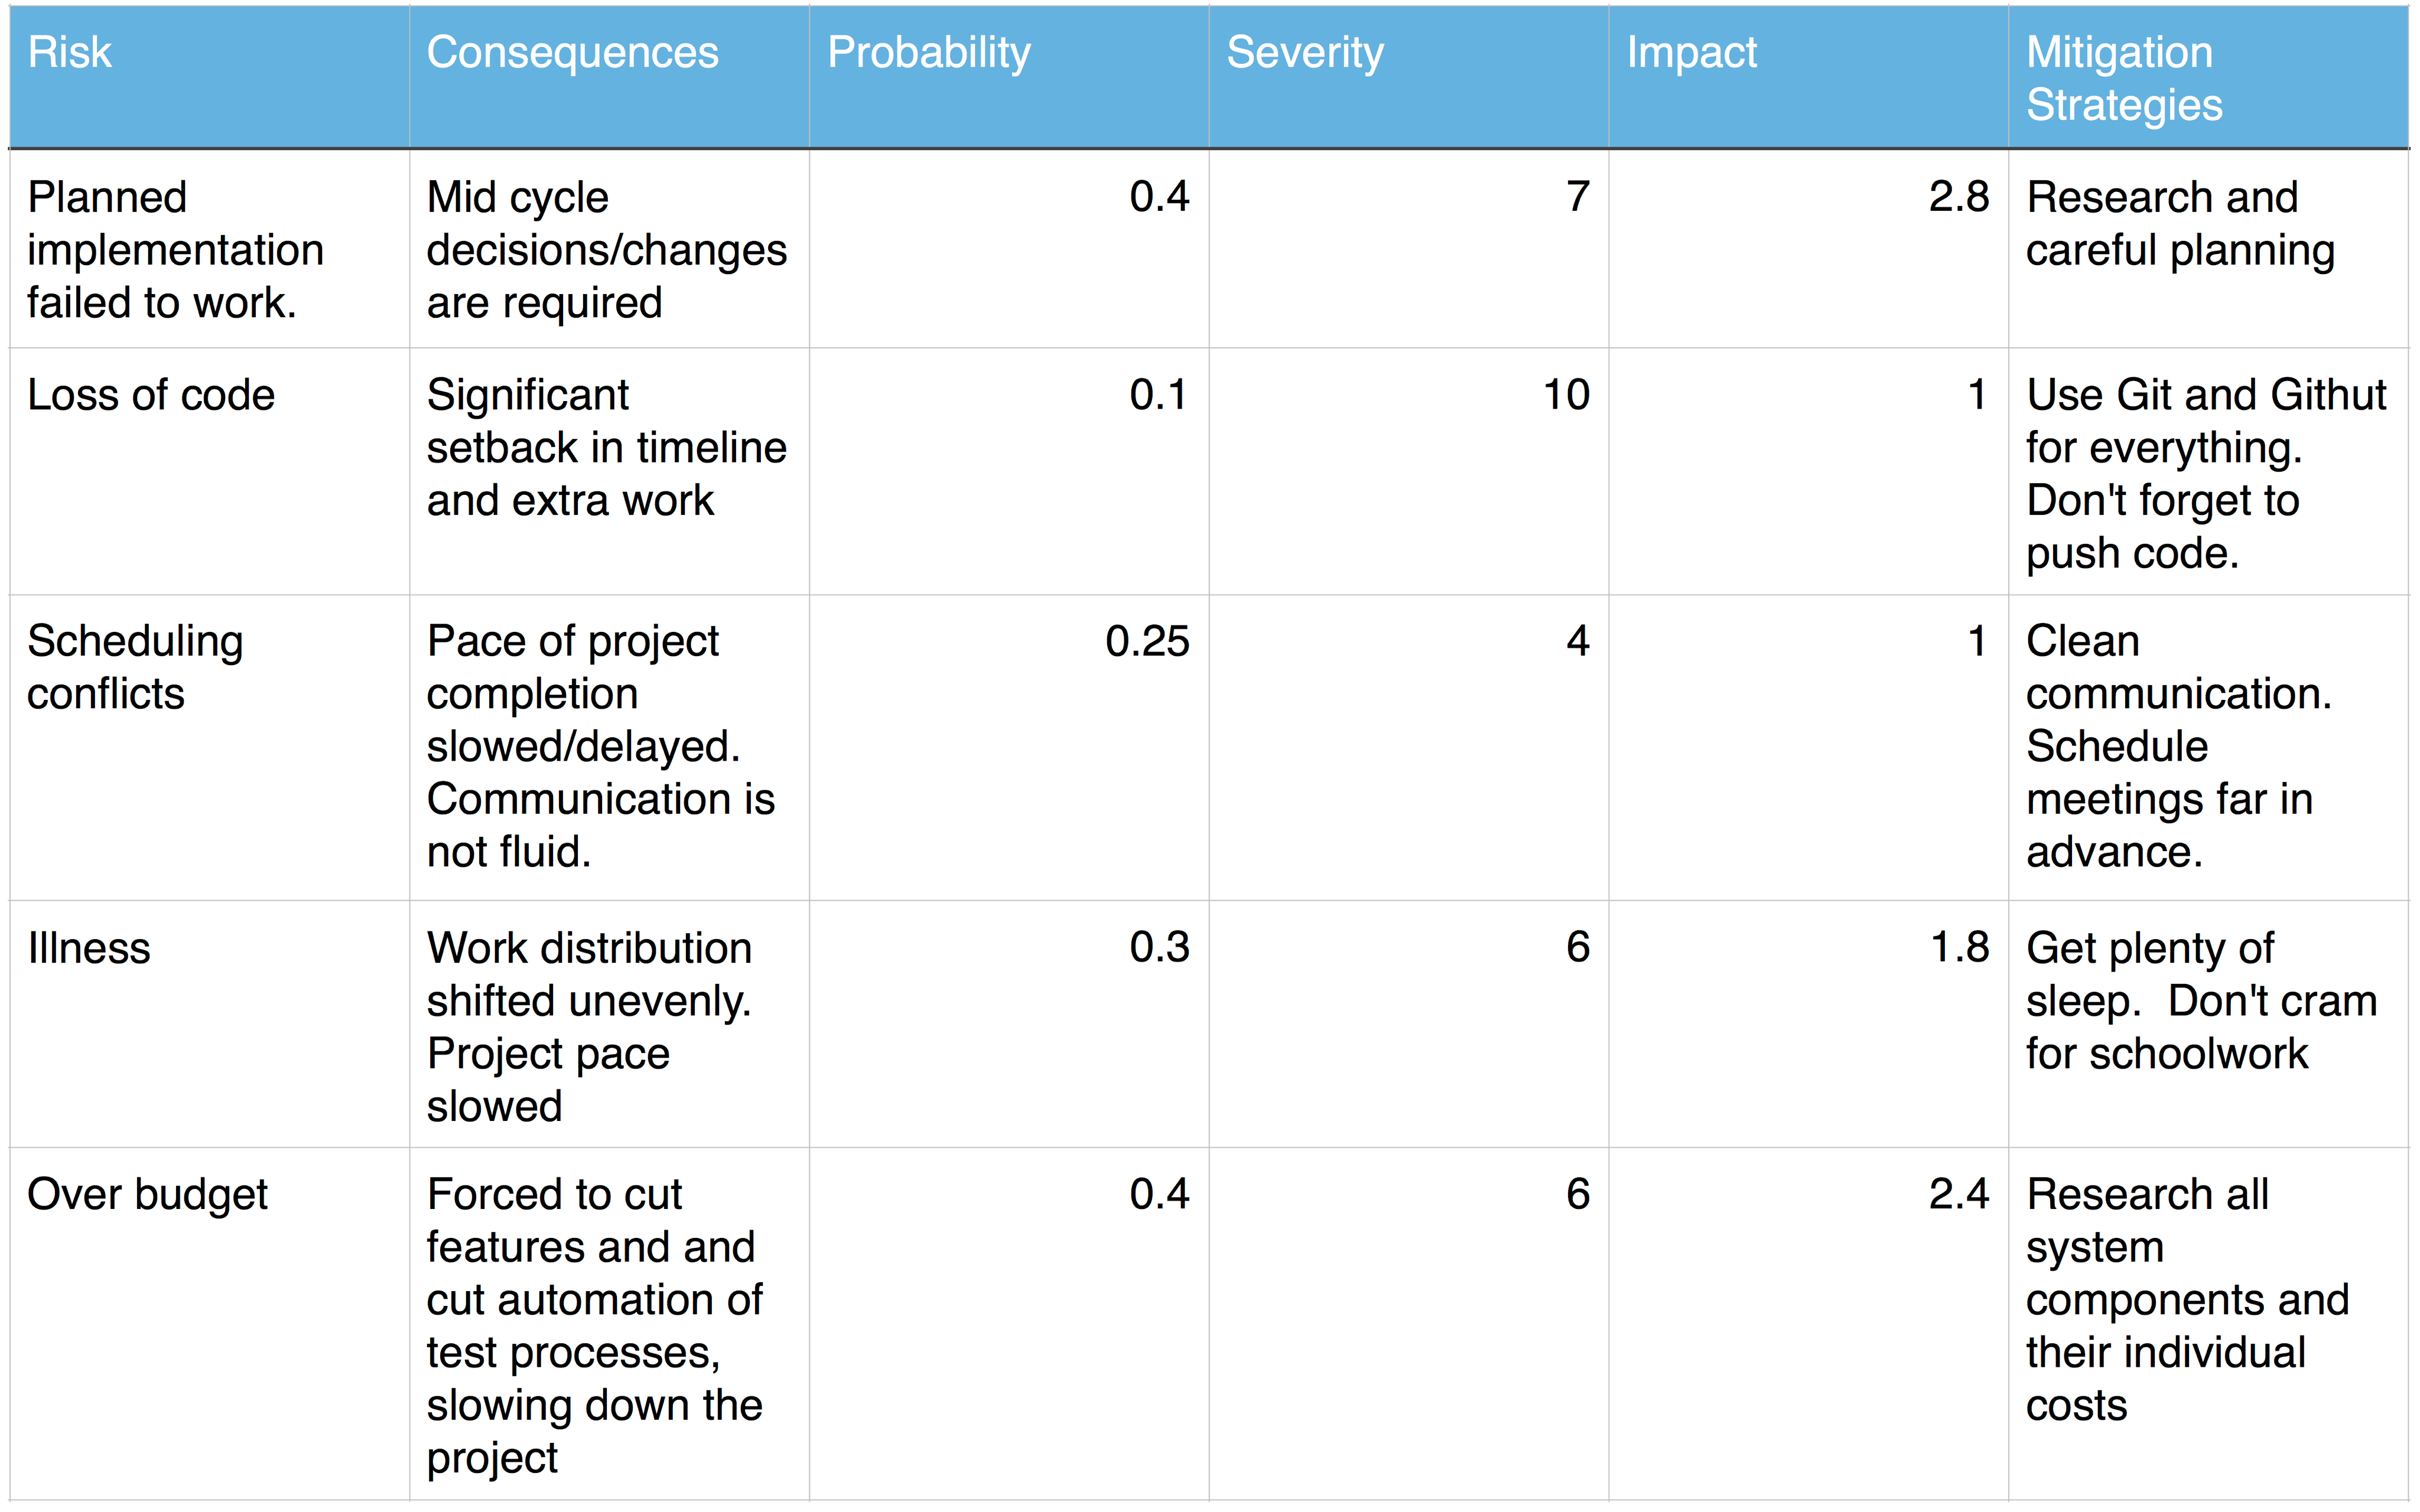
\includegraphics[width=1\textwidth]{images/risk.png}
\caption{Risk Analysis Table}
\end{figure}

\begin{figure}
The Development Timeline is a graphical representation of all the tasks that are needed for the completion of the project. This graphical model is known as Gantt Chart.
\newline
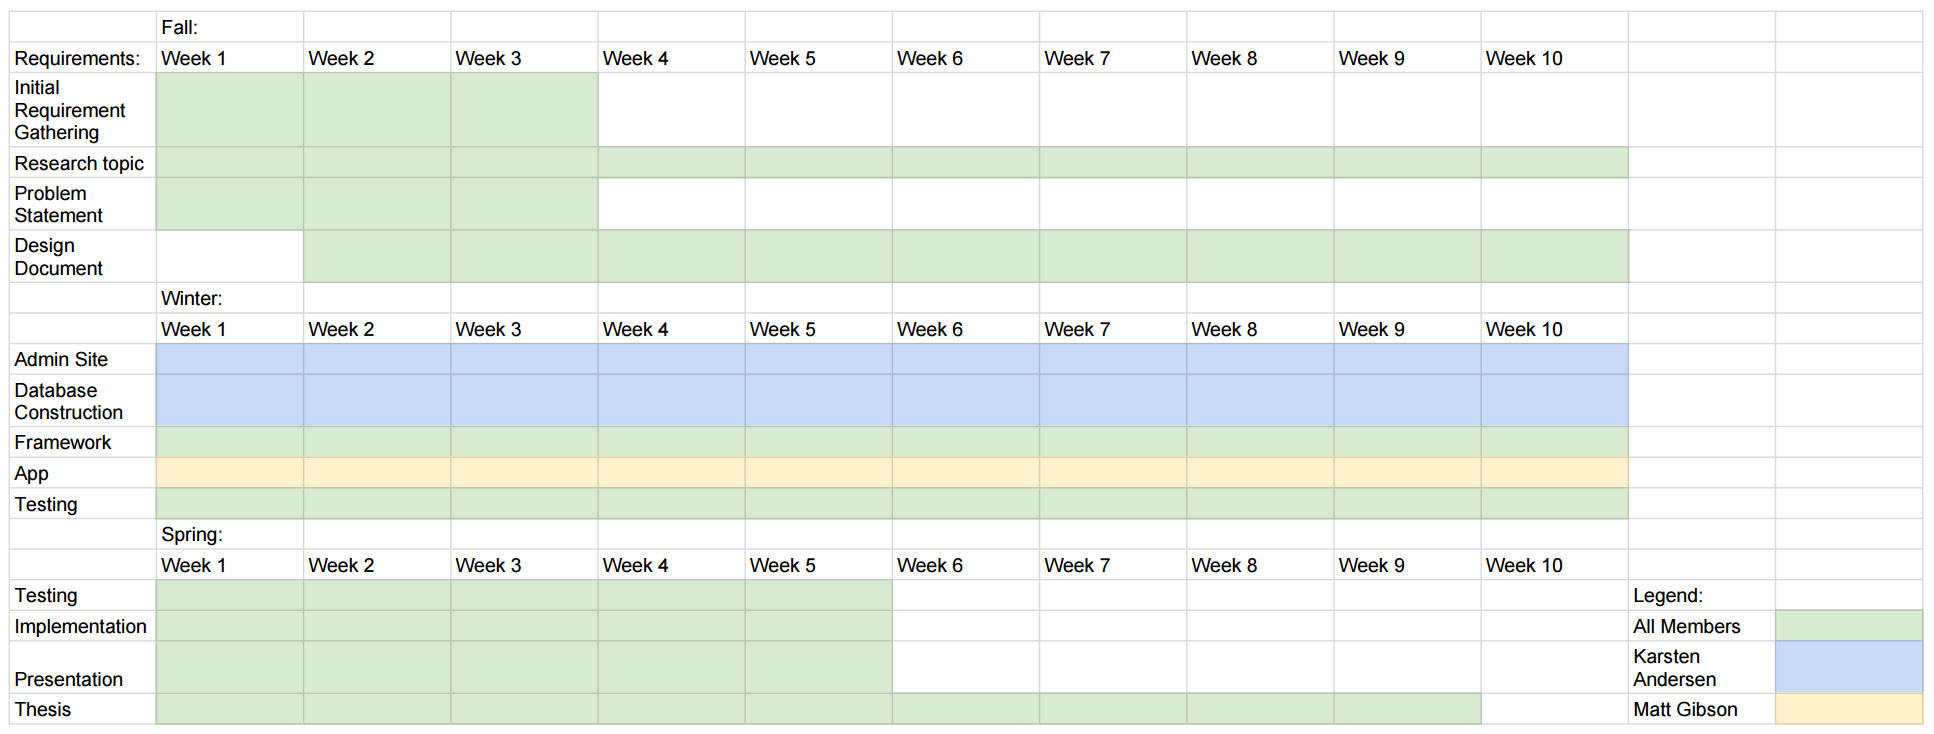
\includegraphics[width=1\textwidth]{images/gantt.png}
\caption{Gantt Chart}
\end{figure}

\section{\\Title of Appendix B}
% the \\ insures the section title is centered below the phrase: Appendix B

\begin{figure}
\chapter{Conceptual Model}
The conceptual model displays examples of our framework in use by an app. This specific one is taking place in a mall.
\newline
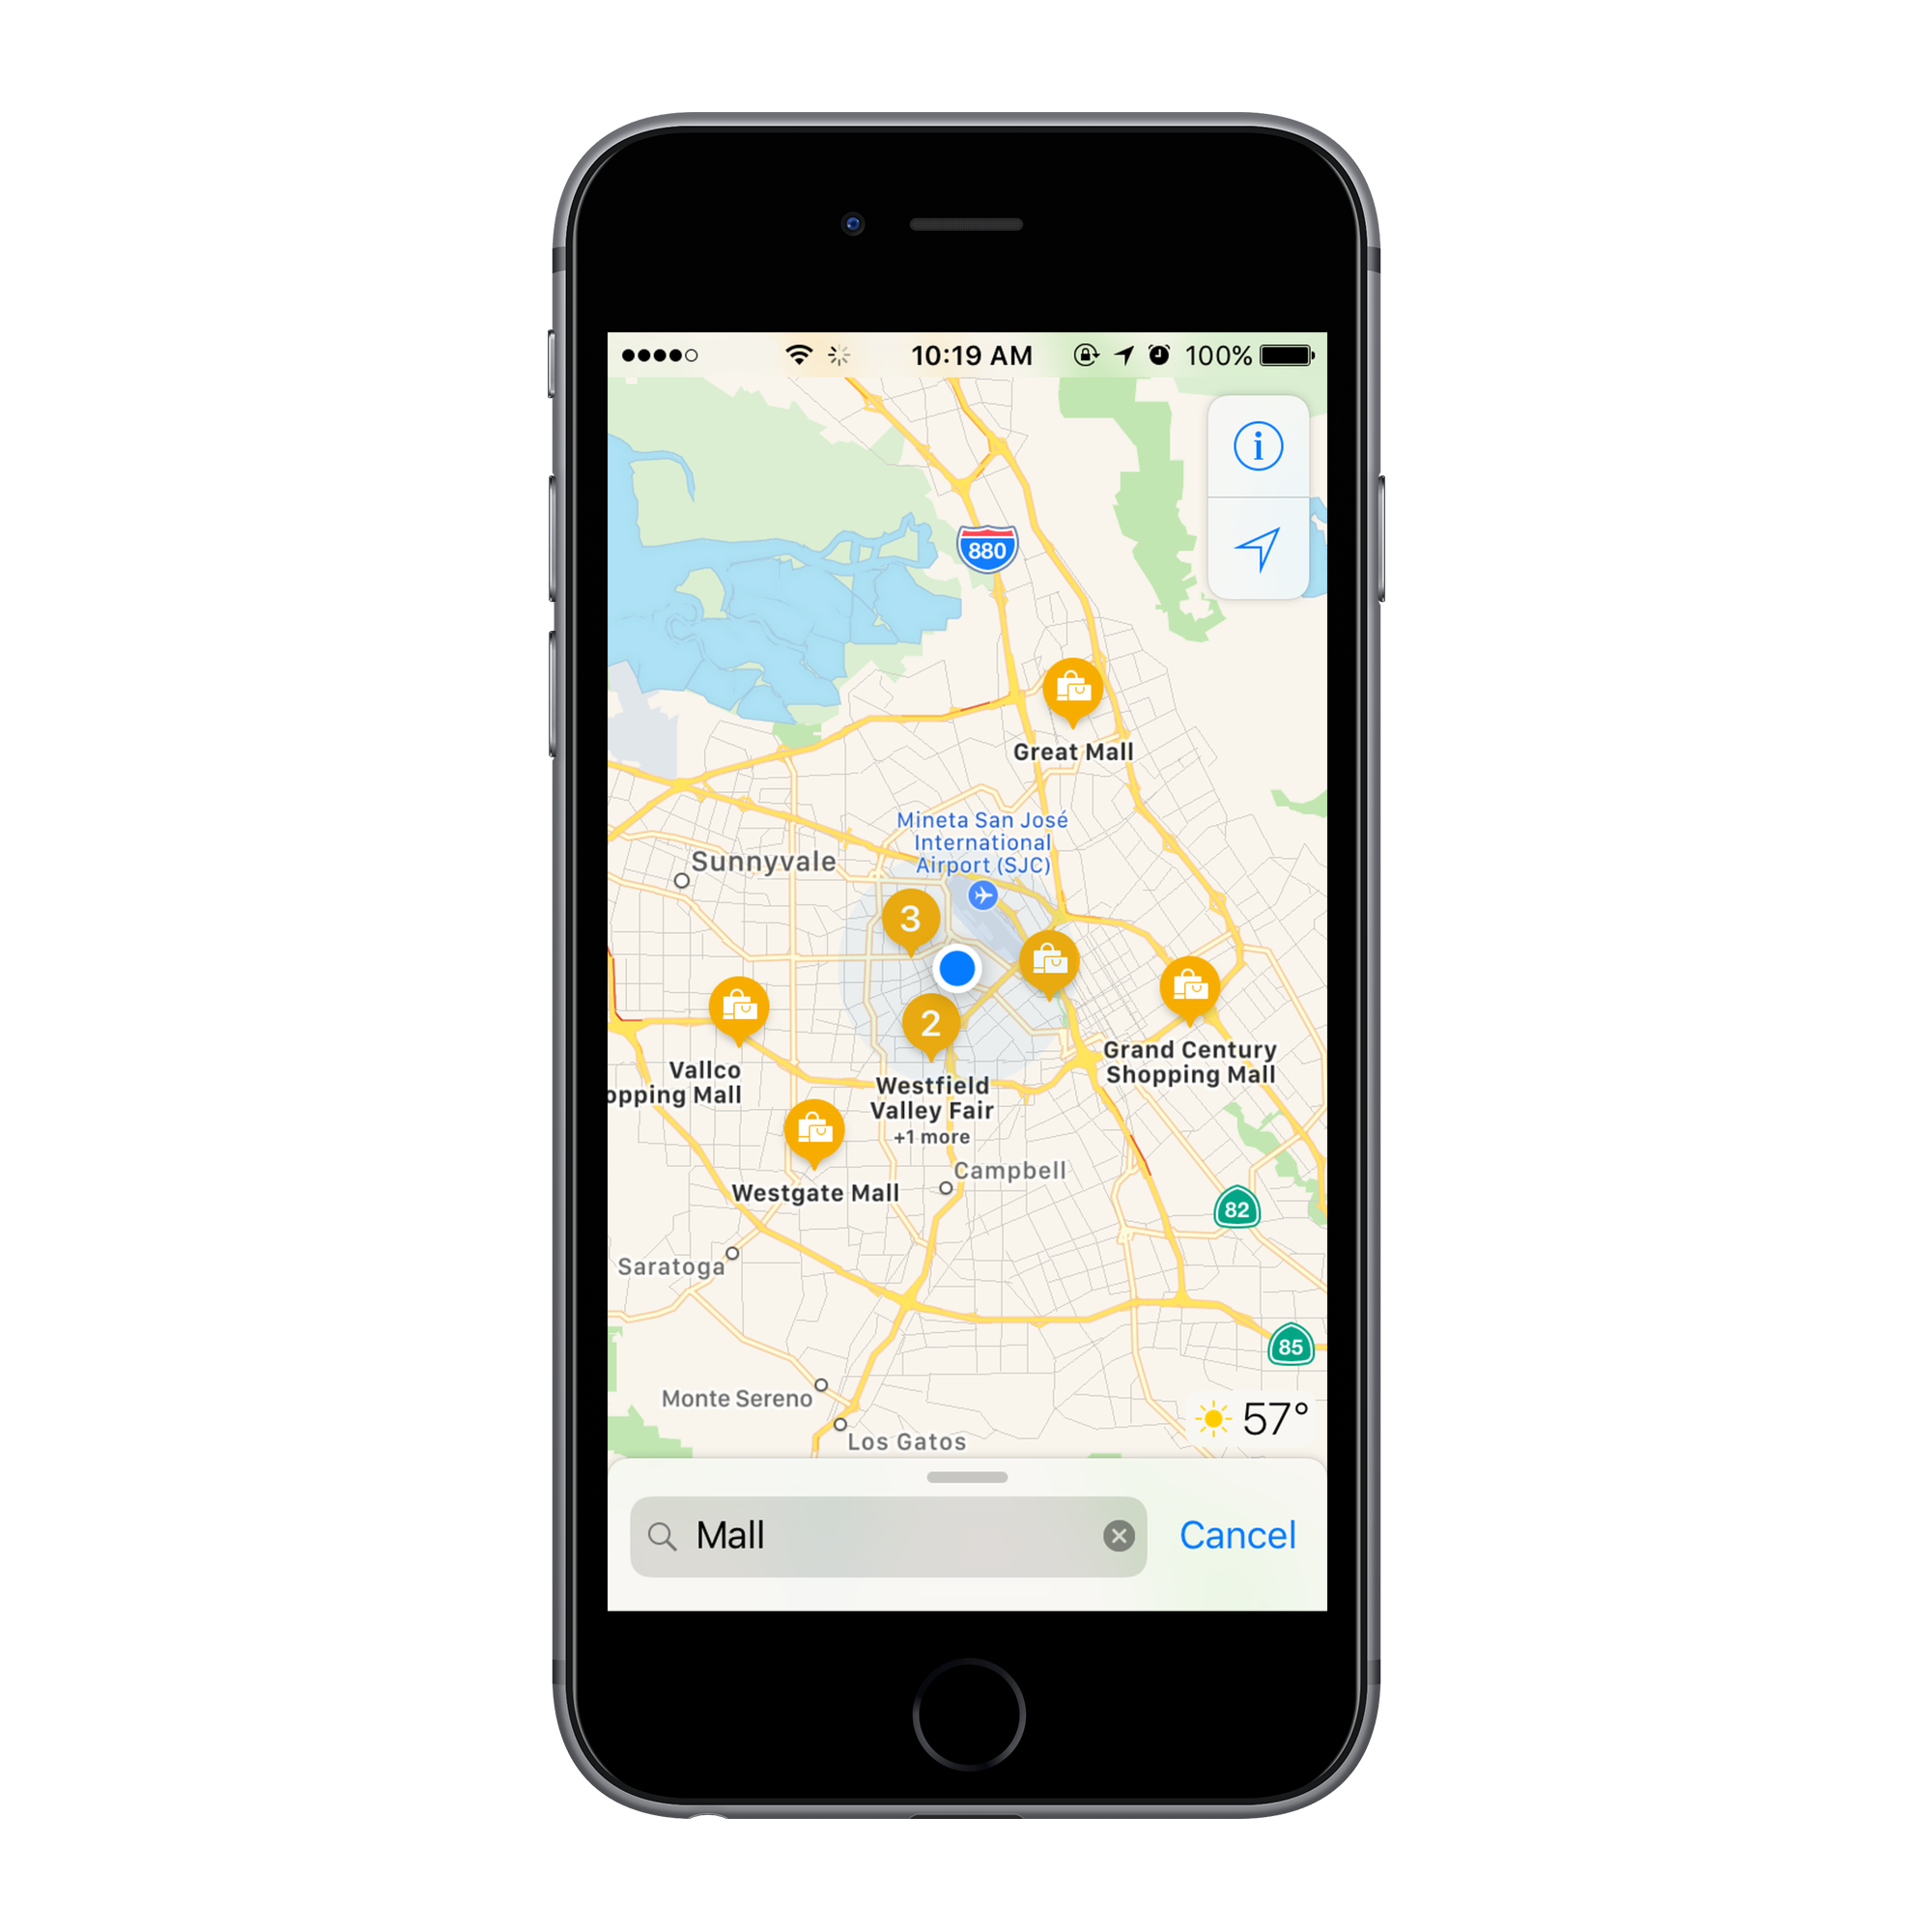
\includegraphics[width=1\textwidth]{images/con1.png}
\caption{Discovering Beacons View}
This is an example of what it would look like while the device is finding bluetooth beacons
\end{figure}
\begin{figure}
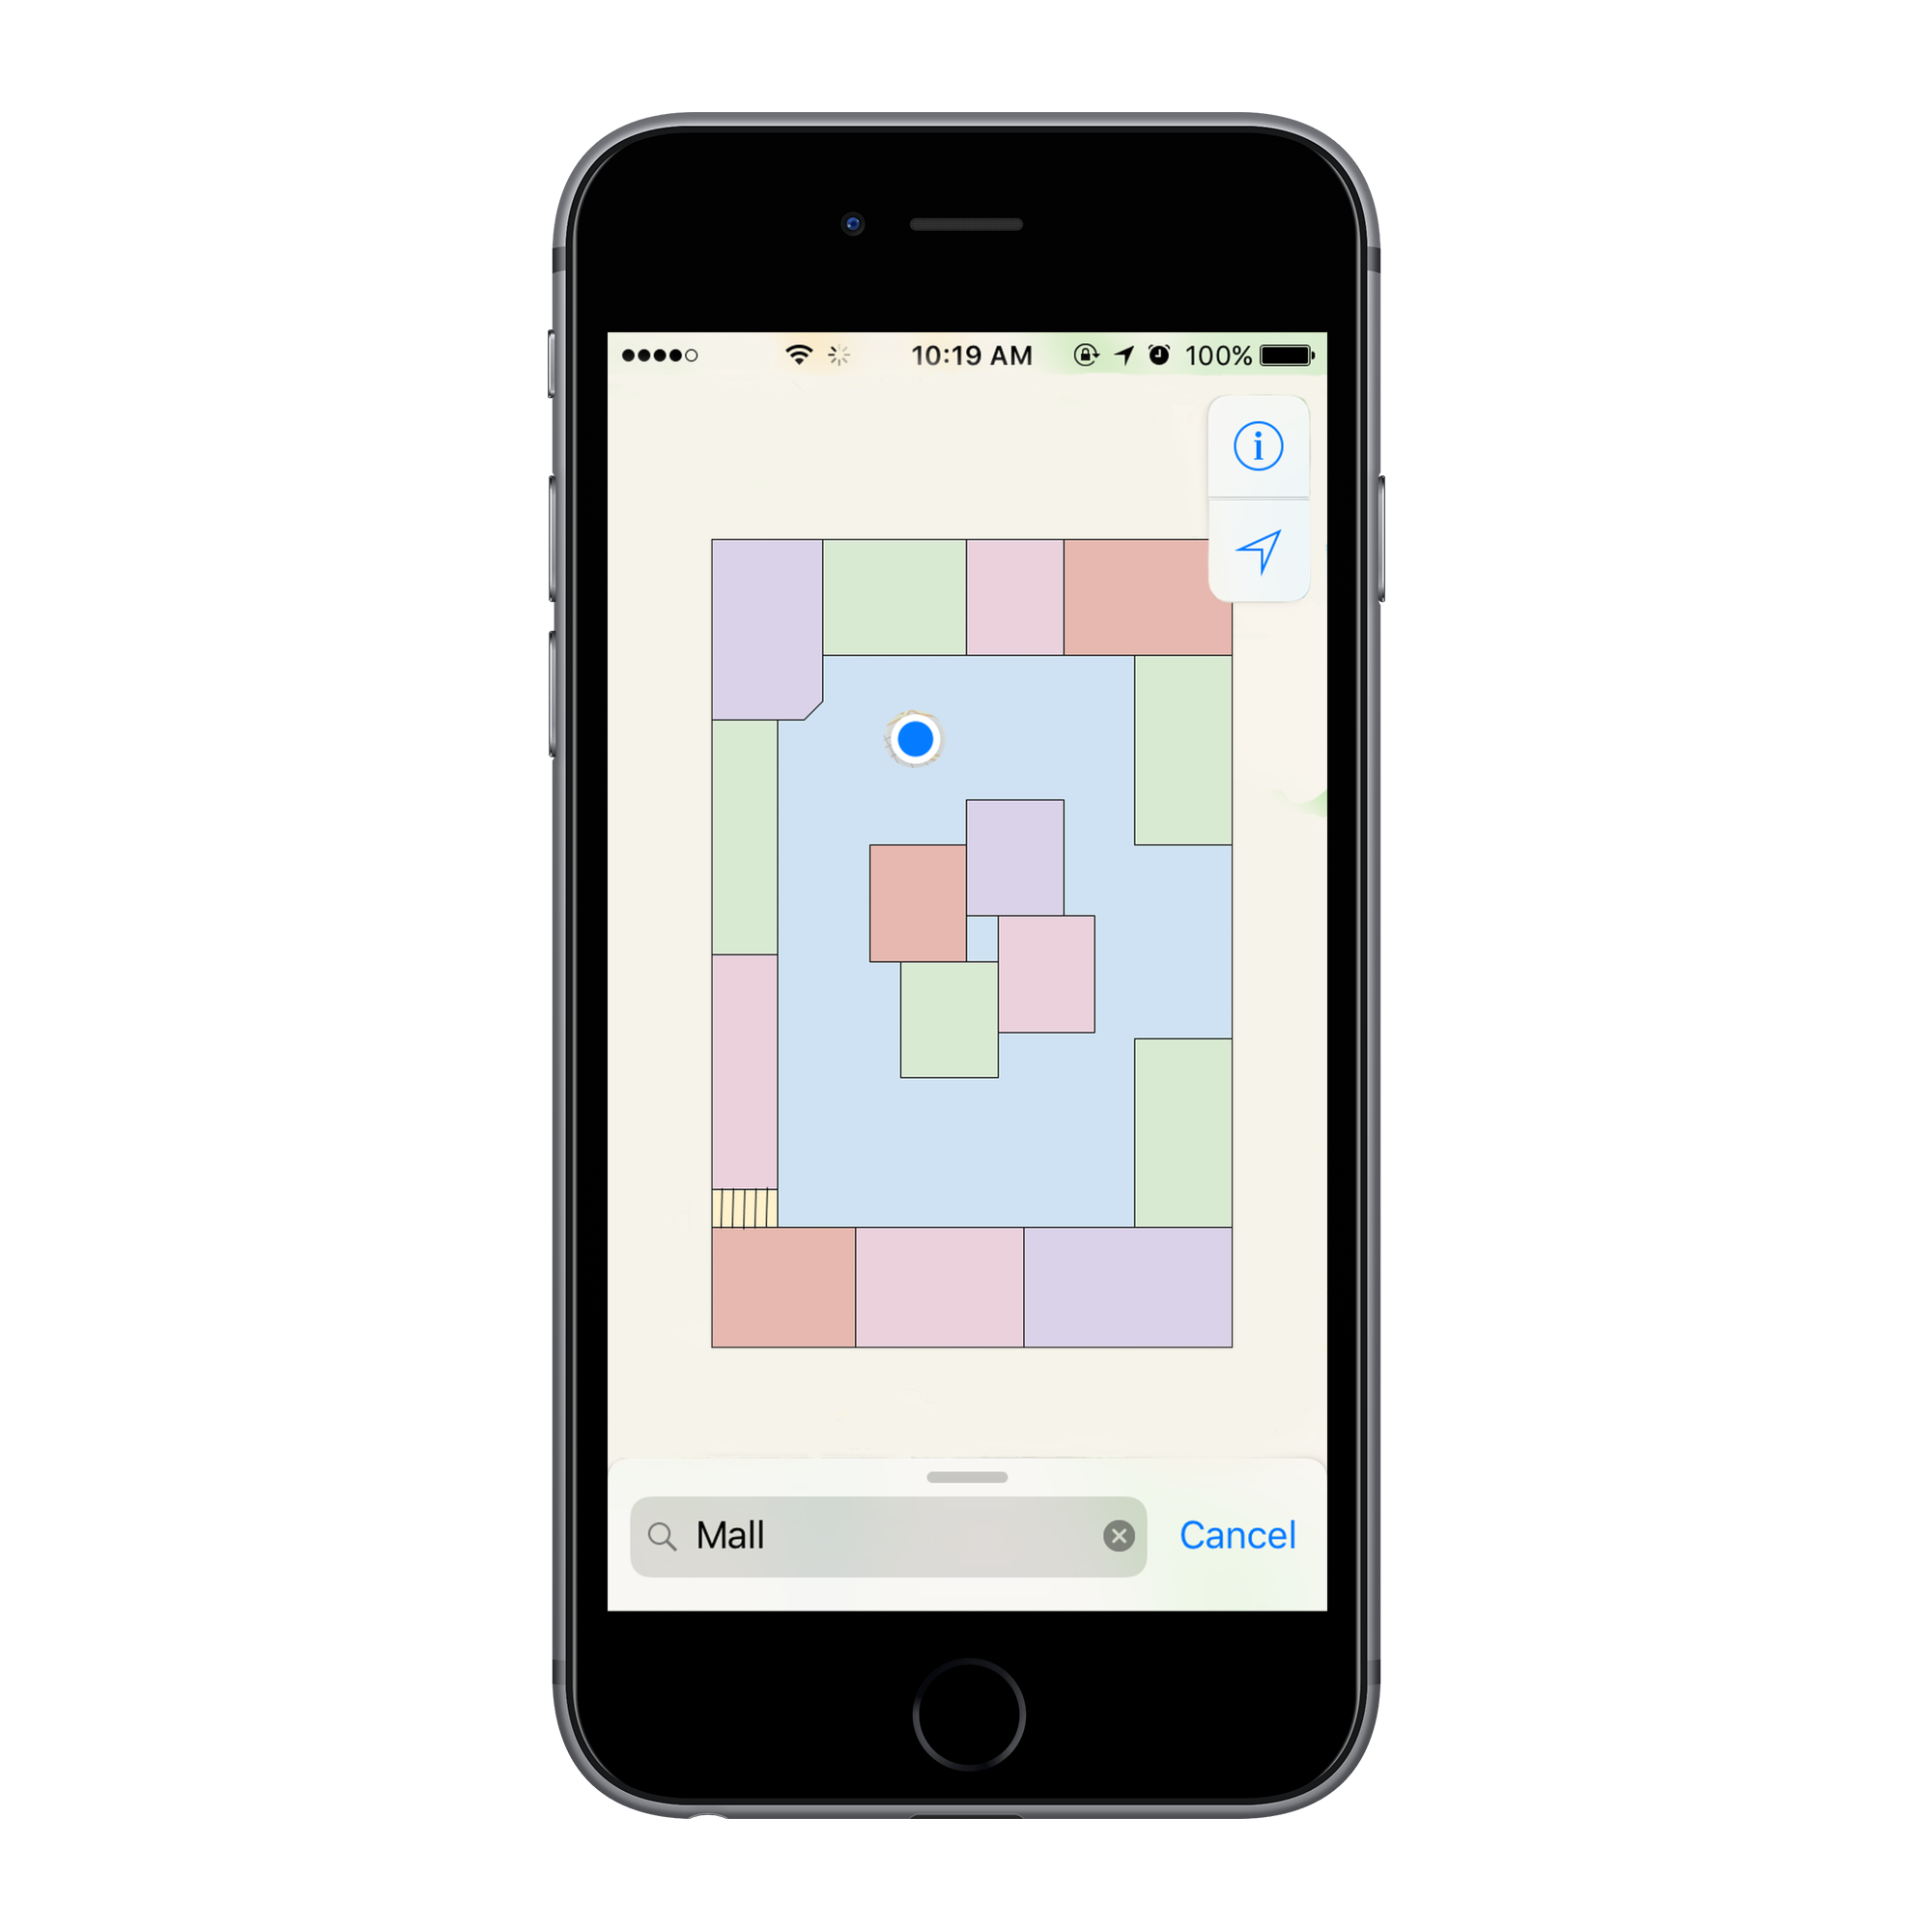
\includegraphics[width=1\textwidth]{images/con2.png}
\caption{Location View}
This is an example of what it would look like while the device is displaying relative location
\end{figure}
